\documentclass{article}
\usepackage[polish]{babel}
\usepackage[T1]{fontenc}
\usepackage{geometry}
\usepackage{chngpage}
\usepackage{graphicx}
\usepackage{subcaption}
\usepackage{algorithm2e}
\usepackage{amsfonts}
\graphicspath{ {./plots/} }
\geometry{margin=2cm}
\usepackage[utf8]{inputenc}
\usepackage{indentfirst}
\usepackage{longtable}
\author{Nie interesuj się}
\title{\vspace{-2.0cm}Sprawozdanie}
\frenchspacing
\setlength{\parindent}{2em}
\usepackage{bm}
\newcommand{\mA}{\bm{A}}
\newcommand{\mB}{\bm{B}}
\newcommand{\mC}{\bm{C}}
\newcommand{\mL}{\bm{L}}
\newcommand{\mU}{\bm{U}}
\newcommand{\mZ}{\bm{0}}
\newcommand{\vb}{\bm{b}}
\newcommand{\vx}{\bm{x}}
\newcommand{\R}{\mathbb{R}}

\begin{document}
\maketitle
\section*{Opis Problemu}
 \noindent Zadanie dotyczyło rozwiązania układu równań liniowych następującej postaci:
$$\mA\vx  = \vb$$
dla danej macierzy współczynników $\textbf{A} \in \mathbb{R}^{n \times n}$ i wektora prawych stron $\textbf{b} \in \mathbb{R}^{n}$\\\\
\noindent Macierz \textbf{A} jest macierzą rzadką i blokową o strukturze:
$$
\mA =
\left(\begin{array}{ccccccc}
\mA_1 & \mC_1 & \mZ & \mZ & \mZ & \cdots & \mZ \\
\mB_2 & \mA_2 & \mC_2 & \mZ & \mZ  & \cdots & \mZ \\
\mZ  & \mB_3 & \mA_3 & \mC_3 & \mZ  & \cdots & \mZ \\
\vdots & \ddots & \ddots & \ddots & \ddots & \ddots & \vdots\\
\mZ   & \cdots & \mZ  & \mB_{v-2} & \mA_{v-2} & \mC_{v-2} & \mZ \\
\mZ  & \cdots & \mZ  &  \mZ &\mB_{v-1} & \mA_{v-1} & \mC_{v-1}  \\
\mZ  & \cdots & \mZ & \mZ & \mZ& \mB_{v} & \mA_{v}  \\
\end{array}\right)
$$ 
gdzie $v=\frac{n}{\ell}$ zakładając że $\ell|n$, gdzie $\ell \geq 2$ jest rozmiarem każdej z kwadratowych macierzy wewnętrznych (bloków):
\begin{itemize}
	\item $\mA_k \in \mathbb{R}^{\ell \times \ell}$, $k=1,...,v$ są macierzami gęstymi
	\item $\mB_k \in \mathbb{R}^{\ell \times \ell}$, $k=2,...,v$ są postaci:
	$$
	\mB_k =
	\left(\begin{array}{ccccc}
	0 & \cdots & 0 & b_{1\,\ell-1}^k & b_{1\,\ell}^k \\
	0 & \cdots & 0 & b_{2\,\ell-1}^k & b_{2\,\ell}^k \\
	\vdots & & \vdots & \vdots & \vdots \\
	0 & \cdots & 0 & b_{\ell\,\ell-1}^k & b_{\ell\,\ell}^k \\
	\end{array}\right)
	$$ 
	\item $\mC_k \in \mathbb{R}^{\ell \times \ell}$, $k=1,...,v-1$ są diagonalne:
	$$
	\mC_k =
	\left(\begin{array}{ccccc}
	c_{1}^k & 0 & 0 & \cdots & 0  \\
	0 &  c_{2}^k &  0 & \cdots & 0  \\
	\vdots &  \ddots &  \ddots & \ddots & \vdots  \\
	0 & \cdots & 0 &  c_{\ell-1}^k & 0 \\
	0 & \cdots & 0 &  0 & c_{\ell}^k \\
	\end{array}\right)
	$$
	\item $\mZ \in \mathbb{R}^{\ell \times \ell}$ to macierz zerowa
\end{itemize}
\noindent W celu rowiązania układów równań liniowych $\mA\vx  = \vb$ użyte zostaną cztery metody:
\begin{itemize}
	\item Eliminacji Gaussa bez wyboru elementu głównego
	\item Eliminacji Gaussa z wyborem elementu głównego
	\item Obliczyć $\mL\mU$ macierzy $\mA$ bez wyboru elementu głównego, a następnie obliczyć $\mL\mU\vx = \vb$
	\item Obliczyć $\mL\mU$ macierzy $\mA$ z wyborem elementu głównego, a następnie obliczyć $\mL\mU\vx = \vb$
\end{itemize}
\newpage
\section*{Efektywne przechowywanie macierzy rzadkiej}
W konstruowaniu rozwiązania niezwykle istotny był odpowiedni sposób przechowywania macierzy w pamięci, ponieważ naiwne przechowywanie przykładowej macierzy o krawędzi $n=50000$ będzie niemożliwe ze względu na ograniczoną pamięć.\\

\noindent Zważywszy na to że $\mA$ jest macierzą rzadką -  posiada tylko $n\ell+3(n-\ell)$ elementów niezerowych:
\begin{itemize}
	\item $\ell^2$ w każdym z $v$ bloków $\mA_k$
	\item $2\ell$ w każdym z $v-1$ bloków $\mB_k$
	\item $\ell$ w każdym z $v-1$ bloków $\mC_k$
\end{itemize}
Istnieje sposób na efektywne przechowywanie tylko niezerowych elementów macierzy. Jest to możliwe przy pomocy dostępnej w języku \textit{julia} struktury \textit{\textbf{SparseMatrixCSC}}. Przechowuje ona poszczególne wartości macierzy skompresowane (tylko niezerowe wartości są przechowywane) w porządku kolumnowym. W związku z tym, że algorytm eliminacji Gaussa ma przebieg wierszowy, zdecydowałem się także na transpozycję macierzy (dzięki transpozycji czas dostępu do elementów jest krótszy).
\section*{Metoda eliminacji Gaussa - Teoria}
W sposobie rozwiązywania równań liniowych tą metodą, wyróżnić można dwa etapy: \\\\ \indent Pierwszy etap polega na doprowadzeniu układu do układu równoważnego z macierzą trójkątną górną. Zasada działania tej części algorytmu sprowadza się do zerowania kolejnych elementów znajdujących się pod diagonalą. Przykładowo w celu wyzerowania elementu $a_{i1}$ od i-tego wiersza zostanie odjęty pierwszy wiersz pomnożony przez $\frac{a_{i1}}{a_{11}}$ (\textit{mnożnik}). W analogiczny sposób wyzerowane zostają wszystkie elementy poniżej pierwszego wiersza w pierwszej kolumnie, następnie poniżej drugiego wiersza w drugiej kolumnie itd. Warty zauważenia jest fakt, że do poprawnego działania, algorytm ten wymaga aby żaden z elementów na diagonali nie był zerem. Aby algorytm mógł działać poprawnie również w takiej sytuacji, konieczna jest możliwość zamiany miejscami wierszy.\\\\
\indent Drugi etap to zastosowanie algorytmu \textit{podstawiania wstecz}, ktory opiera się na obliczeniu 
$$x_i = \frac{b_i - \sum^{n}_{j=i+1}a_{ij}}{a_{ii}}$$
dla kolejnych $i$-tych wierszy, rozpocznając od ostatniego z nich.\\\\
\indent Algorytm eliminacji gaussa ma złożoność $O(n^3)$, a algorytm postawiania wstecz - $O(n^2)$. Złożoność całego rozwiązania wynosi więc $O(n^3)$.
\section*{Metoda eliminacji Gaussa - Implementacja}
\noindent \textbf{Opis}\\\\
\indent W sposobie rozwiązania uwzględniona została specyficzna, trójdiagonalno-blokowa postać macierzy $\mA$. Oto graficzne przedstawienie przykładowej macierzy $\mA$ o dowolnym $n$ podzielnym przez 4, oraz $\ell=4$:
$$
\left(\begin{array}{ccccccccc}
a_{1\,1}^1 & a_{1\,2}^1 & a_{1\,3}^1 & a_{1\,4}^1 & c_{1\,1}^1 & 0 & 0 & 0 & \cdots \\
a_{2\,1}^1 & a_{2\,2}^1 & a_{2\,3}^1 & a_{2\,4}^1 & 0 & c_{2\,2}^1 & 0 & 0 & \cdots \\
a_{3\,1}^1 & a_{3\,2}^1 & a_{3\,3}^1 & a_{3\,4}^1 & 0 & 0 & c_{3\,3}^1 & 0 & \cdots \\
a_{4\,1}^1 & a_{4\,2}^1 & a_{4\,3}^1 & a_{4\,4}^1 & 0 & 0 & 0 & c_{3\,3}^1 & \cdots \\
0 & 0 & b_{1\,1}^2 & b_{1\,2}^2 & a_{1\,1}^2 & a_{1\,2}^2 & a_{1\,3}^2 & a_{1\,4}^2 & \cdots \\
0 & 0 & b_{2\,1}^2 & b_{2\,2}^2 & a_{2\,1}^2 & a_{2\,2}^2 & a_{2\,3}^2 & a_{2\,4}^2 & \cdots \\
0 & 0 & b_{3\,1}^2 & b_{3\,2}^2 & a_{3\,1}^2 & a_{3\,2}^2 & a_{3\,3}^2 & a_{3\,4}^2 & \cdots \\
0 & 0 & b_{4\,1}^2 & b_{4\,2}^2 & a_{4\,1}^2 & a_{4\,2}^2 & a_{4\,3}^2 & a_{4\,4}^2 & \cdots \\
0 & 0 & 0 & 0 & 0 & 0 & b_{1\,1}^3 & b_{1\,1}^3 & \cdots \\
\vdots & \vdots & \vdots & \vdots & \vdots & \vdots & \vdots & \vdots & \ddots \\
\end{array}\right)
$$
\newpage
Jak można zauważyć, nie jest konieczne zerowanie wszystkich elementów znajdujących się pod diagonalą. Dla pierwszych $\ell-2$ kolumn niezerowe elementy mogą znajdować się jedynie w pierwszych $\ell$ rzędach ($\mA_1$), dla $2\ell-2$ kolumn w pierwszych $2\ell$ rzędach ($\mB_2$ oraz $\mA_2$) itd. Schemat jest powtarzalny, daje więc możliwość na wyprowadzenie ogólnego wzoru na indeks ostatniego niezerowego elementu w danej kolumnie \textit{column}:
$$
lastRow(column) = \min\left\lbrace n,~\ell + \ell \cdot \left \lfloor\frac{column + 1}{\ell}\right \rfloor\right\rbrace
$$
\indent Poza ostatnimi $\ell$ wierszami, w każdym wierszu ostatni element należy zawsze do diagonali macierzy blokowej $\mC_i$. Te elementy znajdują się zawsze w odległości $\ell$ od właściwej diagonali $\mA$. W ostatnich $\ell$ rzędach to $\mA_v$ jest leżącym najbardziej z prawej strony blokiem, a więc ostatnie niezerowe elementy leżą na kolumnie $n$-tej. Stąd wzór na ostatni niezerowy element w rzędzie \textit{row}:
$$
lastColumn(row) = \min\{n,~row + \ell\}.
$$
\indent Dodatkowym faktem wartym zauważenia jest brak jakichkolwiek nowych elementów niezerowych nad diagonalą bloków $\mC_i$, co pozwala nam zoptymalizować algorytm \textit{podstawiania wstecz} tak by sumować tylko elementy do kolumny określonej powyższym wzorem na ostatnią kolumnę ($last(row)$).\\\\
\noindent \textbf{Analiza złożoności}\\\\
\indent Przy założeniu że $\ell$ jest stałą, złożoność obliczeniowa zmodyfikowanej metody wynosi $O(n)$ - liczba przebiegów wszystkich pętli to $(n-1)*2\ell*\ell+n*\ell$.\\\\
\noindent \textbf{Algorytm}\\\\
\rule{\textwidth}{0.4pt}
\begin{algorithm}[H]
	\KwData{\\$A$ - macierz\\
		$b$ - wektor prawych stron macierzy A\\
		$n$ - rozmiar macierzy A\\
		$\ell$ - rozmiar bloku macierzy wewnetrznych w A\\}
	\KwResult{\\$x$ - wektor długości n zawierający rozwiązanie $Ax=b$\\
		$it$ - licznik iteracji}
	\vspace{0.3cm}
	$it \gets 0$\\
	\For {$k \gets 1$ \textbf{to} $n-1$ }{
		\For {$i \gets k+1$ \textbf{to} $\min\left\lbrace n,~\ell + \ell \cdot \left \lfloor\frac{k + 1}{\ell}\right \rfloor\right\rbrace$ }{
			\If {$|A[k,k] = 0$} {
				\Return  Error - Na diagonali znajduje się zero.
			}
			$mult \gets \frac{A[k,i]}{A[k,k]}$\\
			$A[k,i] \gets 0$\\
			\For {$j \gets k+1$ \textbf{to} $\min\{n,~k + \ell\}$ }{
				$A[j,i] \gets A[j,i] - mult*A[j,k]$\\
				$it \gets it+1$\\
			}
		$b[i] \gets b[i] - mult*b[k]$
		}
	}
	\For {$i \gets n$ \textbf{downto} $1$ }{
		\For {$j \gets k+1$ \textbf{to} $\min\{n,~i + \ell\}$ }{
			$sum \gets sum + x[i] * A[j,i]$\\
		}
	$x[i] \gets \frac{b[i] -sum}{A[i,i]}$\\
	}
	\Return x, it
\end{algorithm}
\hrule
\newpage
\section*{Wariant eliminacji Gaussa z częściowym wyborem elementu głównego}
\noindent \textbf{Opis}\\\\
W sytuacji gdy nie możemy zastosować poprzedniego algorytmu (zero na diagonali $\mA$), musimy zastosować jego inny wariant, który pozwala na rozwiązywanie takich układów.\\
\indent Zasada działania jest prosta - wybrany zostaje wiersz, dla którego element w eliminowanej kolumnie k ma największą bezwzględną wartość i zostaje on zamieniony z k-tym wierszem. Dalsza eliminacja przebiega bez zmian.\\
\indent W związku z dużym kosztem takiego rozwiązania, stosuję dodatkowy wektor $p$ służący do przechowywania informacji o pozycji danego wiersza w macierzy.\\\\
\noindent \textbf{Algorytm}\\\\
\rule{\textwidth}{0.4pt}
\begin{algorithm}[H]
	\KwData{\\$A$ - macierz\\
		$b$ - wektor prawych stron macierzy A\\
		$n$ - rozmiar macierzy A\\
		$\ell$ - rozmiar bloku macierzy wewnetrznych w A\\}
	\KwResult{\\$x$ - wektor długości n zawierający rozwiązanie $Ax=b$\\
		$it$ - licznik iteracji}
	\vspace{0.3cm}
	$it \gets 0$\\
	$p \gets \{i : i \in \{1, \ldots, n \} \}$\\
	\For {$k \gets 1$ \textbf{to} $n-1$ }{
		\For {$i \gets k+1$ \textbf{to} $\min\left\lbrace n,~\ell + \ell \cdot \left \lfloor\frac{k + 1}{\ell}\right \rfloor\right\rbrace$ }{
			$max\_row \gets k$\\
			$max = |A[k,p[k]]|$\\
			\For {$j \gets i$ \textbf{to} $\min\left\lbrace n,~\ell + \ell \cdot \left \lfloor\frac{k + 1}{\ell}\right \rfloor\right\rbrace$ }{
				\If {$|A[k,p[j]]| > max$}{
					$max\_row \gets j$\\
					$max \gets |A[k,p[j]]|$\\
					$it \gets it+1$\\
				}
			}
			\If {$|max| = 0$} {
				\Return  Error - macierz osobliwa.
			}
			$p[k], p[max\_row] \gets p[max\_row], p[k] $\\
			$mult \gets \frac{A[k,p[i]]}{A[k,p[k]]} $\\
			$A[k,p[i]] \gets 0$\\
			\For {$j \gets k+1$ \textbf{to} $\min\left\lbrace n,~2\ell + \ell \cdot \left \lfloor\frac{k + 1}{\ell}\right \rfloor\right\rbrace$ }{
				$A[j,p[i]] \gets A[j,p[i]] - mult* A[j,p[k]]$\\
				$it \gets it+1$\\
			}
		$b[p[i]] \gets b[p[i]] - mult* b[p[k]] $
		}
	}
	\For {$i \gets n$ \textbf{downto} $1$ }{
		\For {$j \gets k+1$ \textbf{to} $\min\left\lbrace n,~2\ell + \ell \cdot \left \lfloor\frac{p[i] + 1}{\ell}\right \rfloor\right\rbrace$ }{
			$sum \gets sum + x[j] * A[j,p[i]]$\\
		}
		$x[i] \gets \frac{b[p[i]] -sum}{A[i,p[i]]}$\\
	}
	\Return x, it
\end{algorithm}
\hrule
\newpage
\noindent \textbf{Analiza złożoności}\\\\
\indent Podstawową różnicą między tą a poprzednią wersją algorytmu, jest szersze oszacowanie możliwego położenia ostatniego niezerowego elementu w rzędzie:
$$
lastColumn(row) = \min\left\lbrace n,~2\ell + \ell \cdot \left \lfloor\frac{row + 1}{\ell}\right \rfloor\right\rbrace
$$
Analogicznie do poprzedniej metody, także tutaj możemy zauważyć że w trakcie eliminacji $\ell-2$ pierwszych kolumn najdalszy niezerowy element można stworzyć w kolumnie $2\ell$ itd.\\\\
\indent Zmiany te zmieniają jednak tylko stałe, więc ogólna złożoność pozostaje $O(n)$
\section*{Rozkład LU}
\noindent \textbf{Teoria}\\\\
\indent Rozkład $\mL\mU$ macierzy $\mA$ to przedstawienie zadanej macierzy w postaci iloczynu $\mA=\mL\mU$, gdzie $\mL$ jest macierzą trójkątną dolną, a $\mU$ jest macierzą trójkątną górną. Dodatkowo, elementy na diagonali $\mL$ mają wartość 1. \\\\
\indent Do uzyskania rozkładu $\mL\mU$ ponownie użyłem metody eliminacji Gaussa - macierz $\mA$ zostaje przekształcona do macierzy górnotrójkątnej ($\mU$), a macierz $\mL$ jest uzyskana poprzed zapamiętywanie mnożników użytych do przekształceń (mnożnik $mult_{j,i}$ służący do wyzerowania elementu $a_{j,i}$ bedzie zapisany w $L[j,i]$). Zważywszy na duży rozmiar macierzy i cechy rozkładu $\mL\mU$, zapisywany on będzie na jednej macierzy o rozmiarze oryginalnej macierzy $\mA$.\\\\
\indent Przeprowadzenie rozkładu $\mL\mU$ ma złożoność $O(n^3)$, jednakże sposób ten umozliwia znacząco szybsze rozwiązywanie układów w których macierz pozostaje taka sama, a zmienia się jedynie wektor prawych stron. W takim przypadku rozwiązanie sprowadza się jedynie do rozwiązania układu:
$$
\left\{ \begin{array}{l}
\mL\bm{z} = \vb\\
\mU\vx = \bm{z}
\end{array} \right.
$$
Co dzięki trójkątnej postaci macierzy $\mL$ i $\mU$ możemy wykonać w $O(n^2)$ (algorytm postawiania wstecz) \\\\
\noindent \textbf{Opis algorytmów}\\\\
Algorytm przeprowadzający rozkład $\mL\mU$ jest analogiczny do już przeanalizowanych algorytmów - eliminacji gaussa oraz eliminacji gaussa z częściowym wyborem elementu głównego. Jedyna różnica to:
\begin{itemize}
	\item W algorytmie bez wyboru elementu głównego - zamiast zerowania elementów $a_{ij}$ przypisywana jest im wartość mnożnika ($mult = \frac{A[j,i]}{A[j,k]}$)
	\item W algorytmie z wyborem elementu głównego - zamiast zerowania elementów $a_{ij}$ przypisywana jest im wartość mnożnika ($mult = \frac{A[j,p[i]]}{A[j,p[j]]}$)
\end{itemize} 
\noindent \textbf{Analiza złożoności}\\\\
Złożoność jest taka sama jak w przypadku zmodyfikowanej eliminacji gaussa $O(n)$ (przy założeniu że $\ell$ jest stałą), gdzie wersja z częściowym wyborem elementu głównego różni się o stałą.
\newpage 
\section*{Rozwiązanie układu równań z LU}
Rozwiązanie układu:
$$
\left\{ \begin{array}{l}
\mL\bm{z} = \vb\\
\mU\vx = \bm{z}
\end{array} \right.
$$ 
składa się z dwóch etapów:
\begin{enumerate}
	\item rozwiązanie $\mU\vx = \bm{z}$ to omawiany już wcześniej algorytm podstawiania wstecz, indeks ostatniej niezerowej kolumny w wierszu przedstawia się wzorem:
	$$lastColumn(row) = \min\{n,~row + \ell\}$$
	\item rozwiązanie $\mL\bm{z} = \vb$ to algorytm podstawiania w przód, w przeciwieństwie do algorytmu podstawiania wstecz zaczyna on iterację od pierwszego elementu i sumuje coraz dalsze kolumny a nie coraz wcześniejsze. Indeks pierwszej kolumny można wyznaczyć wzorem:
	$$	firstColumn(row) = \max\left\lbrace 1,~\ell \cdot \left \lfloor\frac{row - 1}{\ell}\right \rfloor-1\right\rbrace$$
\end{enumerate}
\noindent \textbf{Analiza złożoności}\\\\
W związku z tym że rozwiązanie to ma tyle samo przebiegów pętli jak część podstawiania wstecz w algorytmach eliminacji gaussa, także tu złożoność wynosi $O(n)$\\\\
\noindent \textbf{Algorytm}\\\\
Przestawiony algorytm dotyczy metody bez wyboru elementu głównego, w algorytmie z wyborem jedyną różnicą jest odwoływanie się do wektora permutacji $p$ zamiast do konkretnego wiersza.\\\\
\rule{\textwidth}{0.4pt}
\begin{algorithm}[H]
	\KwData{\\$A$ - macierz\\
		$b$ - wektor prawych stron macierzy A\\
		$n$ - rozmiar macierzy A\\
		$\ell$ - rozmiar bloku macierzy wewnetrznych w A\\}
	\KwResult{\\$x$ - wektor długości n zawierający rozwiązanie $Ax=b$\\
		$it$ - licznik iteracji}
	\vspace{0.3cm}
	$it \gets 0$\\
	
	\For {$i \gets 1$ \textbf{to} $n$ }{
		$sum \gets 0$\\
		\For {$j \gets \max\left\lbrace 1,~\ell \cdot \left \lfloor\frac{i - 1}{\ell}\right \rfloor-1\right\rbrace$ \textbf{to} $i-1$ }{
			$sum \gets sum + z[j] * A[j,i]$\\
		}
		$z[i] \gets b[i] -sum$\\
	}
	\For {$i \gets n$ \textbf{downto} $1$ }{
		$sum \gets 0$\\
		\For {$j \gets k+1$ \textbf{to} $\min\{n,~i + \ell\}$ }{
			$sum \gets sum + x[i] * A[j,i]$\\
		}
		$x[i] \gets \frac{z[i] - sum}{A[i,i]}$\\
	}
	\Return x, it
\end{algorithm}
\hrule
\newpage
\section*{Wyniki}
W celu potwierdzenia poprawności algorytmów wygenerowałem takie wektory prawych stron aby rozwiązaniem układu był zawsze $(1,...,1)^T$. Następnie testowałem algorytmy, mierząc ich średni błąd względny, czas obliczeń, wielkość alokowanej pamięci oraz ilość operacji (średnia z 10 prób). Próby przeprowadzone byłe dla macierzy o $n \in \{16,1000,5000,10000,15000,20000,50000\}$, $\ell=4$ oraz $c_k=2.0$\\\\\\
\noindent \textbf{błędy względne:}
\begin{center}
	\begin{tabular}{|p{1cm}|p{3cm}|p{3cm}|p{3cm}|p{3cm}|p{3cm}|}
		\hline
		\textbf{n} & \textbf{gauss (julia)} & \textbf{gauss} & \textbf{gauss z wyborem} & \textbf{LU bez wyboru} & \textbf{LU z wyborem}  \\
		\hline
		$16$ & $3.754704674e-16$ & $5.453105385e-15$ & $5.003707553e-16$ & $4.574031282e-15$ & $5.064917260e-16$  \\
		\hline
		$1000$ & $2.234004883e-16$ & $7.552064752e-15$ & $2.313956221e-16$ & $1.182375532e-14$ & $2.123111046e-16$ \\
		\hline
		$5000$ & $2.281285449e-16$ & $1.296241376e-14$ & $2.319702017e-16$ & $1.475353849e-13$ & $2.184968556e-16$ \\
		\hline
		$10000$ & $4.076968120e-16$ & $3.673820219e-14$ & $3.773321219e-16$ & $3.630437761e-14$ & $4.469595776e-16$  \\
		\hline
		$50000$ & $---$ & $9.447293155e-14$ & $5.427796231e-16$ & $9.127843964e-14$ & $5.322902898e-16$ \\
		\hline
	\end{tabular}
\end{center}
\vspace{0.8cm}
\noindent \textbf{pobór pamięci :}
\begin{center}
	\begin{tabular}{|p{1cm}|p{3cm}|p{3cm}|p{3cm}|p{3cm}|p{3cm}|}
		\hline
		\textbf{n} & \textbf{gauss (julia)} & \textbf{gauss} & \textbf{gauss z wyborem} & \textbf{LU bez wyboru} & \textbf{LU z wyborem}  \\
		\hline
		$1000$ & $7.641$ MiB & $117.156$ KiB & $125.094$ KiB & $125.125$ KiB & $133.062$ KiB \\
		\hline
		$5000$ & $190.792$ MiB & $585.859$ KiB & $625.000$ KiB & $625.032$ KiB & $664.172$ KiB \\
		\hline
		$10000$ & $763.054$ MiB & $1.144$ MiB & $1.221$ MiB & $1.210$ MiB & $1.301$ MiB  \\
		\hline
		$15000$ & $1.677$  GiB & $1.717$ MiB & $1.831$ MiB & $1.836$ MiB & $1.951$ MiB  \\
		\hline
		$20000$ & $2.690$  GiB & $2.174$ MiB & $2.319$ MiB & $2.321$ MiB & $2.482$ MiB \\
		\hline
	\end{tabular}
\end{center}
\begin{figure}[ht]
	\centering
	\begin{subfigure}{0.8\textwidth}
		\centering
		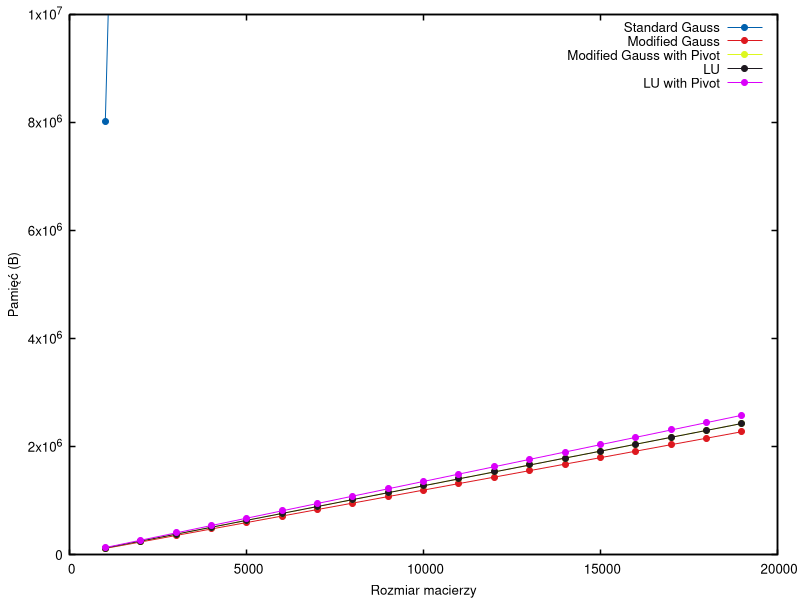
\includegraphics[width=1.0\linewidth]{../plots/plotting_Memory.png}  
	\end{subfigure}
\end{figure} 
\newpage
\noindent \textbf{Różnica dla rozkładów i rozwiązań LU :}\\\\
Pamięć:
\begin{center}
	\begin{tabular}{|p{1cm}|p{3cm}|p{3cm}|p{3cm}|p{3cm}|}
		\hline
		\textbf{n} & \textbf{rozkład LU  bez wyboru} & \textbf{rozwiązanie LU bez wyboru} & \textbf{rozkład LU  z wyborem} & \textbf{rozwiązanie LU z wyborem}  \\
		\hline
		$1000$  & $109.219$ KiB & $15.906$ KiB & $117.156$ KiB & $15.906$ KiB \\
		\hline
		$5000$ & $546.719$ KiB & $78.313$ KiB & $585.859$ KiB & $78.313$ KiB \\
		\hline
		$10000$ & $1.068$ MiB & $156.438$ KiB & $1.144$ MiB & $156.438$ KiB  \\
		\hline
		$15000$ & $1.602$ MiB & $234.563$ KiB & $1.717$ MiB & $234.563$ KiB  \\
		\hline
		$20000$ & $2.029$ MiB & $297.063$ KiB & $2.174$ MiB & $297.063$ KiB \\
		\hline
	\end{tabular}
\end{center}
Czas:
\begin{center}
	\begin{tabular}{|p{1cm}|p{3cm}|p{3cm}|p{3cm}|p{3cm}|}
		\hline
		\textbf{n} & \textbf{rozkład LU  bez wyboru} & \textbf{rozwiązanie LU bez wyboru} & \textbf{rozkład LU  z wyborem} & \textbf{rozwiązanie LU z wyborem}  \\
		\hline
		$1000$  & $0.001404$  & $0.000059$  & $0.001620$  & $ 0.000092$  \\
		\hline
		$5000$ & $0.026826$  & $0.000475$  & $0.029455$  & $0.000552$  \\
		\hline
		$10000$ & $0.150215$  & $0.000794$  & $0.157064$  & $ 0.001153$   \\
		\hline
		$15000$ & $0.330964$  & $0.000948$  & $0.340329$  & $0.001394$   \\
		\hline
		$20000$ & $0.527977$  & $0.001210$  & $0.535301$  & $0.001869$  \\
		\hline
	\end{tabular}
\end{center}
\vspace{0.5cm}
\noindent \textbf{czas obliczeń :}
\begin{center}
	\begin{tabular}{|p{1cm}|p{3cm}|p{3cm}|p{3cm}|p{3cm}|p{3cm}|}
		\hline
		\textbf{n} & \textbf{gauss (julia)} & \textbf{gauss} & \textbf{gauss z wyborem} & \textbf{LU bez wyboru} & \textbf{LU z wyborem}  \\
		\hline
		$1000$ & $0.057868$ & $0.001203$ & $0.001788$ & $0.001463$ & $0.001712$ \\
		\hline
		$5000$ & $0.886813$ & $0.027649$ & $0.029836 $ & $0.027301$ & $0.030007$ \\
		\hline
		$10000$ & $6.801013$ & $0.156763$ & $0.158280$ & $0.151009$ & $0.158218$  \\
		\hline
		$15000$ & $24.141143$ & $0.333071$ & $0.341681$ & $0.330964$ & $0.387559$  \\
		\hline
		$20000$ & $49.588023$ & $0.528979$ & $0.535050$ & $ 0.537977$ & $0.535301$ \\
		\hline
	\end{tabular}
\end{center}
\vspace{-0.3cm}
\begin{figure}[ht]
	\centering
	\begin{subfigure}{0.80\textwidth}
		\centering
		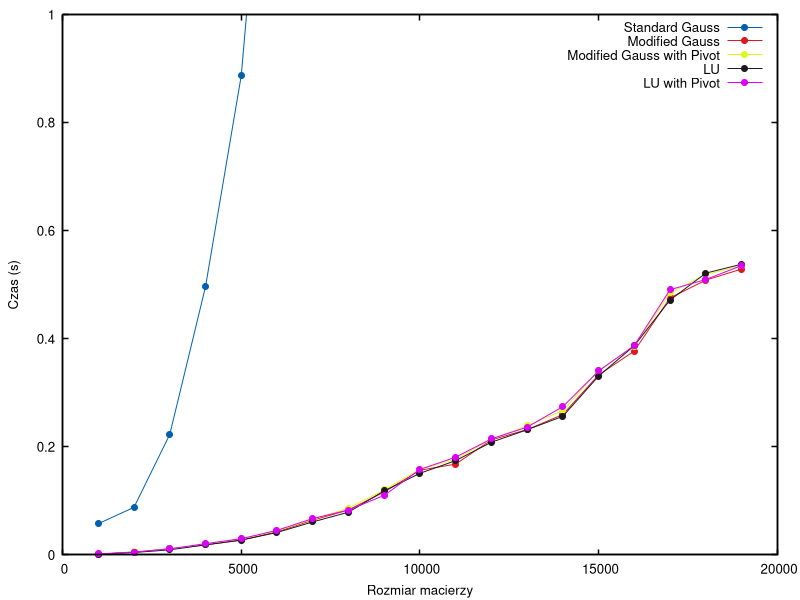
\includegraphics[width=1.0\linewidth]{../plots/plot_time.png}  
	\end{subfigure}
\end{figure}
\newpage
\noindent \textbf{ilość operacji :}
\begin{center}
	\begin{tabular}{|p{1cm}|p{3cm}|p{3cm}|p{3cm}|p{3cm}|}
		\hline
		\textbf{n}  & \textbf{gauss} & \textbf{gauss z wyborem} & \textbf{LU bez wyboru} & \textbf{LU z wyborem}  \\
		\hline
		$1000$ & $13953$ & $27955$ & $17450$ & $31447$ \\
		\hline
		$5000$ & $69958$ & $140388$ & $87450$ & $157880$ \\
		\hline
		$10000$ & $139941$ & $280957$ & $174950$ & $315949$  \\
		\hline
		$15000$ & $209958$ & $421406$ & $262450$ & $473898$  \\
		\hline
		$20000$ & $265963$ & $533996$ & $332450$ & $600488$ \\
		\hline
	\end{tabular}
\end{center}
\begin{figure}[ht]
	\centering
	\begin{subfigure}{0.8\textwidth}
		\centering
		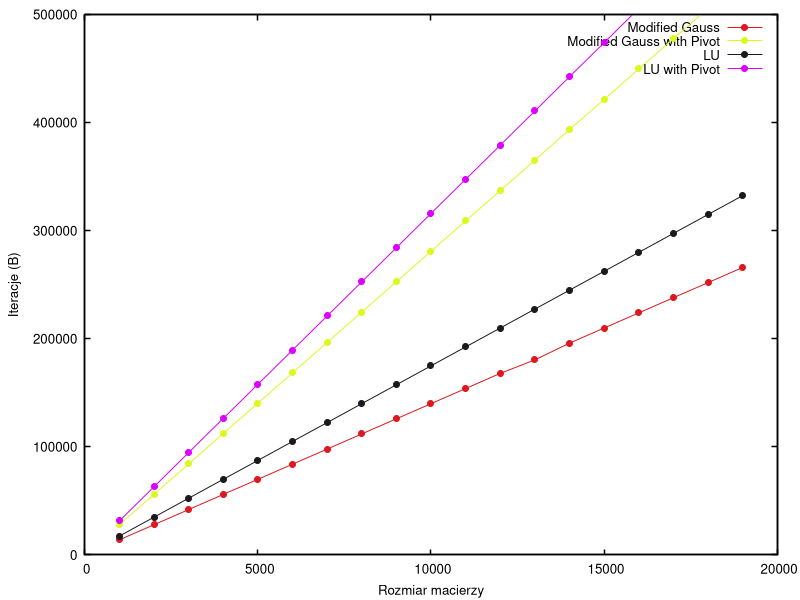
\includegraphics[width=1.0\linewidth]{../plots/plotting_iter.png}  
	\end{subfigure}
\end{figure}
\section*{Obserwacje}
\begin{itemize}
	\item Dla algorytmów z częściowym wyborem elementu głównego błąd względny jest zawsze o przynajmniej rząd wielkości mniejszy niż w ich odpowiednikach bez wyboru.
	\item Złożoność pamięciowa zaimplementowanych metod jest liniowa.
	\item Algorytmy nie używające rozkładu $\mL\mU$ wykorzystują mniej zasobów.
	\item Rozwiązanie układu przy już obliczonym rozkładzie $\mL\mU$ jest wielokrotnie tańsze, zarówno czasowo jak i pamięciowo, niż sam rozkład.
	\item Algorytmy z częściowym wyborem elementu głównego wykonują więcej operacji od ich odpowiedników bez wyboru (mimo to wziąć mają złożoność $O(n)$).
	\item Złożoność czasowa wszystkich zaimplementowanych algorytmów (wszystkie poza \textit{standard gauss}) jest kwadratowa (jest to skutkiem wykorzystania struktury \textit{SparseArrayCSC}, w której dostęp do elementu nie jest tak naprawdę stały).
\end{itemize}
\newpage
\section*{Wnioski}
\begin{itemize}
	\item Przedstawione wyniki zgadzają się z wstępną analizą złożoności algorytmów, według której jest ona liniowa.
	\item Dla osiągnięcia dokładniejszych wyników warto używać metod z częściowym wyborem elementu głównego.
	\item Mimo że dla pojedynczej macierzy algorytm z rozkładem $\mL\mU$ osiąga gorsze wyniki, to jest on opłacalny gdy danej macierzy będziemy używać więcej niż raz (dla różnych wektorów prawych stron).
	\item Dzięki optymalizacji ogólnej postaci algorytmu do konkrentego zastosowania można osiągnąć dużo lepsze wyniki (w tym przypadku zredukować złożoność z $O(n^3)$ do $O(n)$).
\end{itemize}

\end{document}
